% Synthetic fixture: figures drawn in TikZ and pgfplots, listings and pseudocode.
\documentclass{article}
\usepackage[T1]{fontenc}
\usepackage{lmodern}
\usepackage{amsmath}
\usepackage{tikz}
\usepackage{pgfplots}
\pgfplotsset{compat=1.17}
\usepackage{listings}
\usepackage[ruled,vlined]{algorithm2e}
\usepackage{hyperref}

\lstset{basicstyle=\ttfamily\small,breaklines=true}

\title{A Queue That Forgets}
\author{S. Haddad}
\date{}

\begin{document}
\maketitle

\section{Idea}
A queue of fixed length drops its oldest entry when a new one arrives.
Figure~\ref{fig:flow} sketches the flow.

\begin{figure}[ht]
\centering
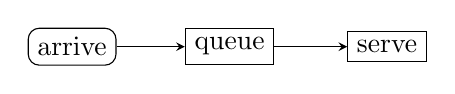
\begin{tikzpicture}[node distance=2cm, >=stealth]
  \node[draw, rounded corners] (in) {arrive};
  \node[draw, right of=in] (q) {queue};
  \node[draw, right of=q] (out) {serve};
  \draw[->] (in) -- (q);
  \draw[->] (q) -- (out);
\end{tikzpicture}
\caption{Entries move from left to right.}\label{fig:flow}
\end{figure}

\section{Measurements}
The mean wait grows with the arrival rate, as Figure~\ref{fig:wait} shows.

\begin{figure}[ht]
\centering
\begin{tikzpicture}
  \begin{axis}[xlabel={rate}, ylabel={wait}, width=0.7\textwidth]
    \addplot coordinates {(1,1.0) (2,1.4) (3,2.2) (4,3.9)};
  \end{axis}
\end{tikzpicture}
\caption{Mean wait against arrival rate.}\label{fig:wait}
\end{figure}

\section{Code}
The core is one function; the call \lstinline|push(q, x % 8)| keeps the index in range,
and \lstinline!q.len! is the length.

\begin{lstlisting}[language=Python]
def push(q, x):
    q.append(x)
    if len(q) > q.size:
        q.pop(0)   # 50% of the time this is a no-op
\end{lstlisting}

\begin{algorithm}[ht]
\caption{Serve one entry}\label{alg:serve}
\KwIn{a queue $Q$}
\KwOut{the oldest entry}
\eIf{$Q$ is empty}{
  \Return{nothing}
}{
  $x \leftarrow$ first entry of $Q$\;
  \Return{$x$}
}
\end{algorithm}

\section{Summary}
The queue is small, and Algorithm~\ref{alg:serve} serves it in constant time.

\end{document}
